\documentclass[addpoints]{exam}

\usepackage{graphicx}
\usepackage{hyperref}
\usepackage{tabularx}

% Header and footer.
\pagestyle{headandfoot}
\runningheadrule
\runningfootrule
\runningheader{CS 440}{Project I}{Fall 2019}
\runningfooter{}{Page \thepage\ of \numpages}{}
\firstpageheader{}{}{}

\qformat{{\large\bf \thequestion. \thequestiontitle}\hfill}
\boxedpoints

\title{Project I: Flight Simulator}
\author{CS 440 Computer Graphics\\Habib University\\Fall 2019}
\date{Due: 18h on Wednesday, 6 November}

\begin{document}
\maketitle
\thispagestyle{empty}

In this project you will implement a flight simulator. High level instructions are provided and you are expected to use your knowledge of math, computer science, and computer graphics to make reasonable implementation decisions.

\begin{questions}

  \titledquestion{Terrain}

  A \textit{height map} is commonly used to generate a \textit{terrain mesh}. A height map is a function that takes in 2 values, e.g. longitude and latitude, and generates a height value, $h$. Write a function to generate a height field over a given area in the $xz$- plane. The function would generate a grid in the given area, triangulate it, and randomly perturb the $y$ coordinate of the grid points.
  \begin{figure}[!h]
    \centering
    \begin{tabular}{cc}
      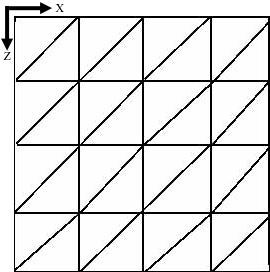
\includegraphics[height=.35\textwidth]{terrain1}
      & 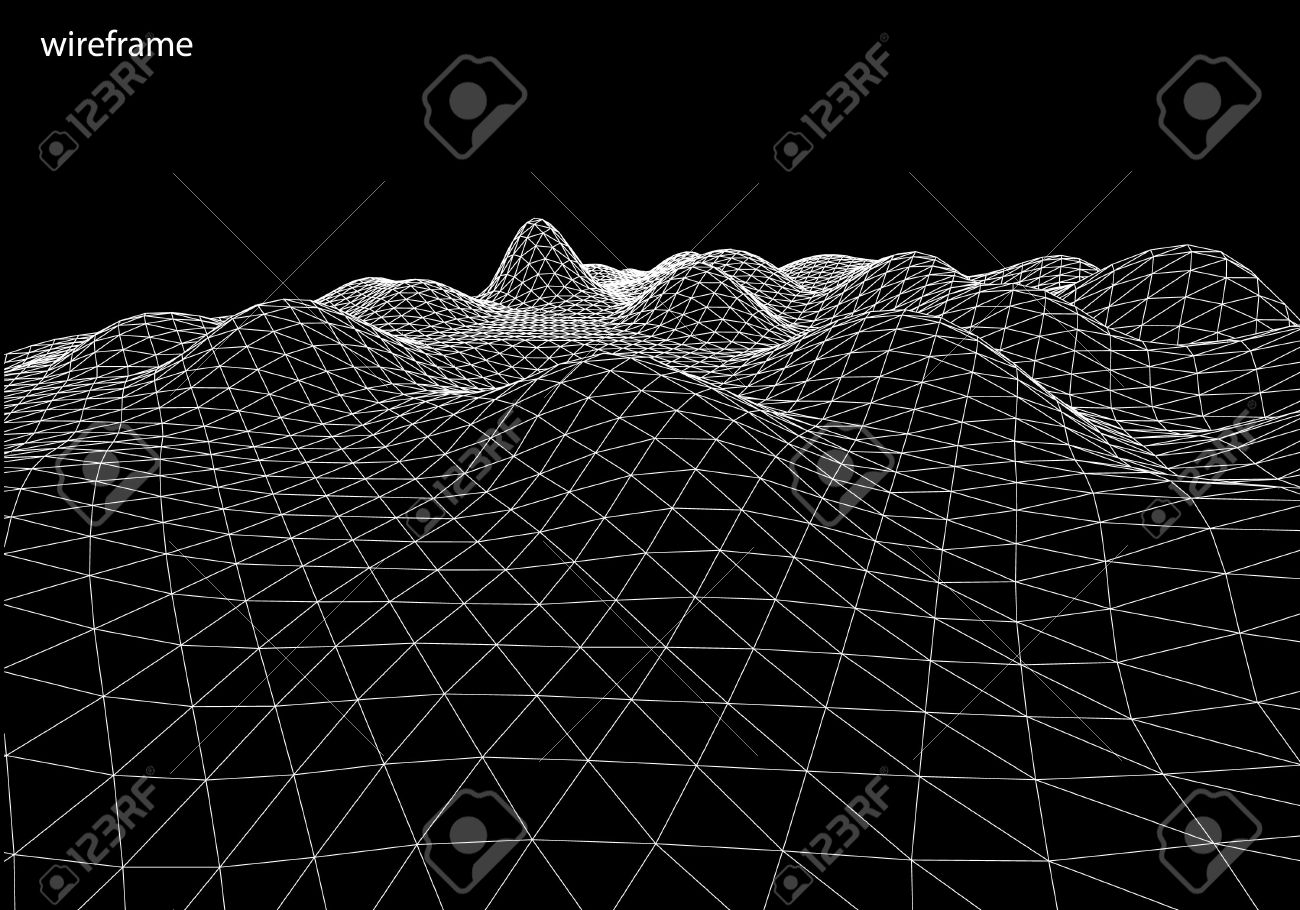
\includegraphics[height=.35\textwidth]{terrain2}\\
      (a) & (b)
    \end{tabular}
    \caption{(a) A triangulated grid in the $xz$- plane. (from \href{http://keithditch.powweb.com/Games/XNA/html/xna\_terrain.html}{Toymaker}) (b) View of an example height field generated by perturbing the $y$- coordinate of the grid points. (from \href{https://www.123rf.com/photo_54102307_stock-vector-3d-wireframe-terrain-contour-vector.html}{123RF})}
  \end{figure}

  \titledquestion{Flight}

  Implement a flyby view of your generated terrain. That is, the perspective view obtained from a plane flying straight ahead at a certain altitude above your terrain and its viewing direction parallel to its direction of movement. Provide mechanisms to dynamically alter the bounds of the view, i.e. \textit{left}, \textit{right}, \textit{top}, \textit{bottom}, \textit{near}, and \textit{far}.

  \titledquestion{To Infinity}

  As the terrain is finite, the plane will ultimately fly out of it. Modify your implementation such that new terrain is dynamically added when the plane approaches the boundary of the existing terrain. This way, the plane never flies out of terrain.

  \titledquestion{Some \href{https://en.wikipedia.org/wiki/Flight_dynamics_(fixed-wing_aircraft)}{Flight Dynamics}}

  The orientation of a plane in flight is determined by its rotation about three axes. The rotations are termed \textit{pitch}, \textit{roll}, and \textit{yaw}, and are illustrated below. Provide mechanisms to accelerate and decelerate the plane, and to vary each of the plane's rotations. Note that the plane's altitude is constrained. It may not descend below or ascend above a certain altitude.

  \titledquestion{Varied Terrain}

  Specify a certain height in your terrain as ground level. Your terrain contains greenery at ground level and the points are colored green. Terrain below ground level is covered by water and the points are colored blue. Only the surface of the water is visible. Terrain above ground level is mountainous and the points are colored green to brown to white as the height increases. Provide mechanisms to switch between viewing the terrain in wire frame, flat shading, and smooth shading.
  \begin{figure}[!h]
    \centering
    \begin{tabular}{cc}
      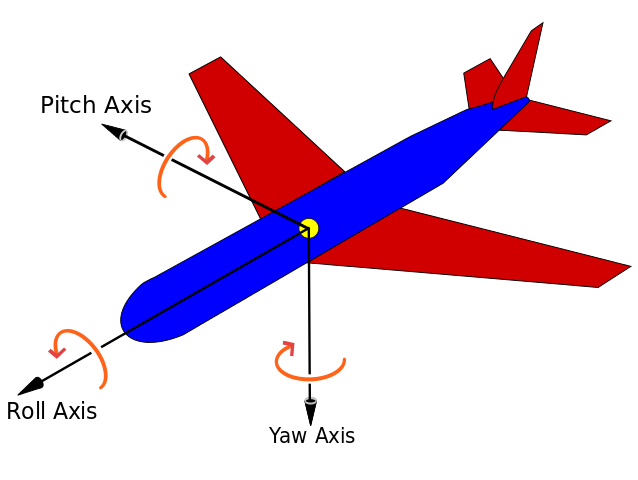
\includegraphics[height=.35\textwidth]{plane}
      &   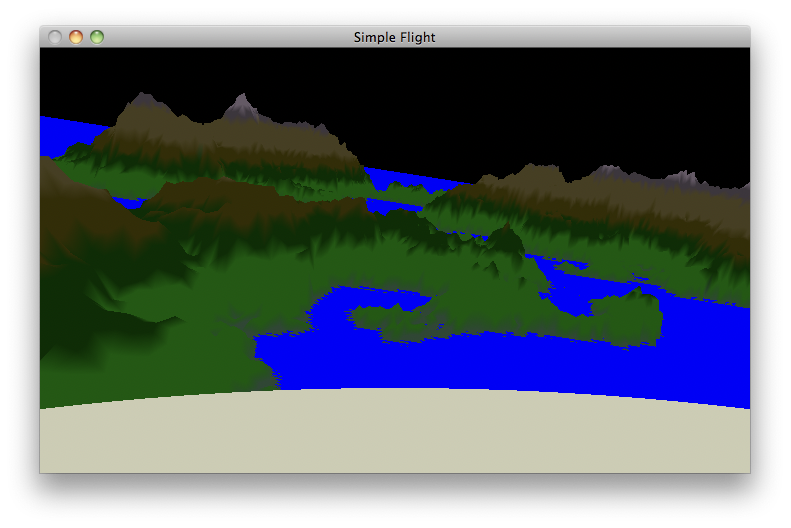
\includegraphics[height=.35\textwidth]{view}\\
      (a) & (b)
    \end{tabular}
    \caption{(a) The three rotations of a plane. (from \href{https://en.wikipedia.org/wiki/Flight_dynamics_(fixed-wing_aircraft}{Wikipedia}) (b) An example view of the terrain. Your view need not contain the dashboard.}
  \end{figure}

  \titledquestion{Freak Out (Bonus)}
  You can include the following additional functionality for a bonus.
  \begin{itemize}
  \item The height map is not completely random but is sensitive to neighboring points thus yielding a smoother terrain.
  \item The height field is read in from an image, e.g. as described \href{http://www.cs.cmu.edu/~jkh/462_s07/assts/assignment1/}{here}.
  \item Implement view dependent shading of the terrain, i.e. the shade assigned to geometry is not constant, rather it varies depending on the viewing direction.
  \item Any other desired functionality.
  \end{itemize}

\end{questions}

\end{document}
%%% Local Variables:
%%% mode: latex
%%% TeX-master: t
%%% End:
